%! TEX root = ../../master.tex
\lecture[Endliche Produkte. Projektionen auf Komponenten. Universelle Eigenschaft des Produkts. Produkte von kompakten und von Hausdorff-Räumen. Diagonaleigenschaft. Unendliche Produkte.]{Do 29 Apr 2021}{Produkte}
\section{Produkte}
\begin{definition}[Produkttopologie]\label{def:produkttopologie}
    Seien $X_1,X_2$ topologische Räume. Die \vocab[Topologie!Produkt-]{Produkttopologie} auf $X_1\times X_2$ ist die Topologie erzeugt von
    \[
    \mathcal{B} = \left \{U_1\times U_2 \mid  U_1\subset X_1 \text{ offen }, U_2\subset X_2\text{ offen}\right\} 
    .\] 
\end{definition}
\begin{example}
    Seien $(X_1,d_1)$ und $(X_2,d_2)$ metrische Räume. Auf $X_1\times X_2$ haben wir die Metriken definiert durch
    \[
        \begin{split}
            d_{\max} ((x_1,x_2),(y_1,y_2) &:= \max \left \{d_1(x_1,y_1), d_2(x_2,y_2)\right\}  \\
            \tilde{d}_1((x_1,x_2),(y_2,y_2)) &:= d_1(x_1,y_1) + d_2(x_2,y_2) \\
            \tilde{d}_2((x_1,x_2),(y_1,y_2)) &:= \sqrt{d_1(x_1,y_1)^2 + d_2(x_2,y_2)^2} 
        \end{split}
    .\] 
    Dies Metriken sind paarweise äquivalent (leicht zu prüfen). Zudem sind $ε$-Bälle in  $d_{\max}$ gegeben durch
    \[
        U_{d_{\max}}((x_1,x_2),ε)) = U_{d_1}(x_1,ε) \times U_{d_2}(x_2,ε)
    .\] 
    D.h. die von $d_{\max}$ induzierte Topologie ist die Produkttopologie.
\end{example}
\begin{example}
    Es ist $\R^2 \cong \R \times \R$, wobei wir auf der linken Seite die Standardtopologie und auf der rechten Seite die Proudkttopologie meinen.
\end{example}
\begin{remark}
    $\mathcal{B}$ ist per Definition eine Subbasis der Produkttopologie, in der Tat handelt es sich jedoch sogar um eine Basis:
    \begin{proof}
        Seien $U_1\times U_2$ sowie $V_1\times V_2\in \mathcal{B}$ Basiselemente. Wir stellen fest, dass
        \[
            (U_1\times U_2)\cap (V_1\times V_2) = (U_1\cap U_2) \times (V_1\cap V_2)
        .\] 
        das Produkt zweier Basiselemente ist, und somit sind wir fertig.
    \end{proof}
\end{remark}
\begin{theorem}[Projektion auf Komponenten]\label{thm:projektion-auf-komponente-ist-stetig}
    Die Projektionen
        \begin{equation*}
        p_x: \left| \begin{array}{c c l} 
        X\times Y & \longrightarrow & X \\
        (x,y) & \longmapsto &  x
        \end{array} \right.
        \qquad
        p_Y: \left| \begin{array}{c c l} 
            X\times Y & \longrightarrow & Y \\
            (x,y) & \longmapsto	 &  y
        \end{array} \right.
    \end{equation*}
    sind stetig und offen
\end{theorem}
\begin{proof}
    Sei $U\subset X$ offen. Dann ist $p_X^{-1}(U) = U\times Y\in \mathcal{B}$, also offen. Analoges gilt für $p_Y$. \\
    Sei $U\subset X\times Y$ offen. Dann können wir $U$ schreiben als
     \[
    U = \bigcup_{i \in  I} U_i \times V_i
    .\] 
    OBdA können wir $V_i \neq  \emptyset$ annehmen. Dann ist aber
    \[
        P_X(U) = \bigcup_{i \in  I} p_X(U_i \times V_i) = \bigcup_{i \in  I} U_i \subset X
    .\] 
    offen, also ist $p_X$ offen.
\end{proof}

\begin{recap}
    Was passiert mit der leeren Menge? Hierzu erinnern wir uns an
    \[
        X\times Y \coloneqq  = \left \{(x,y) \mid  x\in X, y\in Y\right\} 
    .\] 
    also
    \[
        X\times \emptyset = \left \{(x,y) \mid  x\in X, y\in \emptyset\right\}  = \emptyset
    .\] 
\end{recap}

\begin{remark}
    Die Projektion $p_X$ ist i.A. nicht abgeschlossen.
     \begin{proof}
         Betrachte $A = \left \{\left( \frac{1}{n},n \right) \in \R^2 \mid  n \in \mathbb{N}_{>0}\right\} \subset \R^2$  abgeschlossen. Dann ist aber $p_1(A) = \left \{\frac{1}{n}\mid n \in \mathbb{N}_{>0}\right\} \subset \R$ \underline{nicht} abgeschlossen.
    \end{proof}
\end{remark}
\begin{theorem}\label{thm:projektion-auf-x-ist-abgeschlossen-wenn-y-kompakt}
    Ist $Y$ kompakt, so ist  $p_X$ abgeschlossen. 
\end{theorem}
\begin{proof}
    Sei $A\subset X\times Y$ abgeschlossen. Wir müssen zeigen, dass $X \setminus p_X(A)$ offen ist, also wähle $x\in X \setminus p_X(A)$. Für alle $y\in Y$ ist $(x,y) \not\in A$ (sonst wäre $x\in p_X(A)$, also gibt es 
    \[
        x\in U_y \subset X \quad y\in V_y \subset Y \text{ offen} \colon (U_y \times V_y) \cap A = \emptyset
    .\] 
    Damit sind die $\left \{V_y\right\} _{y\in Y}$ eine offene Überdeckung von $Y$ und  wir finden mit  $Y$ kompakt eine endliche Teilüberdeckung  $V_{y_1},\ldots,V_{y_n}$ von $Y$. Setzen wir nun
     \[
    U := \bigcap_{i =1}^n U_{y_i} 
    .\] 
    so ist $U\subset X$ offen als endlicher Schnitt und wir stellen mit
    \[
        U\times V_{y_i} \subset U_{y_i}\times V_{y_i}\subset (X\times Y) \setminus A
    .\] 
    fest, dass bereits $U\times Y\subset (X\times Y)\setminus A$ (weil die $V_{y_i}$ bereits $Y$ überdecken). Nun muss aber bereits
     \[
         U\subset X \setminus p_X(A)
    .\] 
    gelten, und damit ist dieses $U$ eine offene Umgebung von  $x\in X \setminus p_X(A)$.
    \begin{figure}[h]
        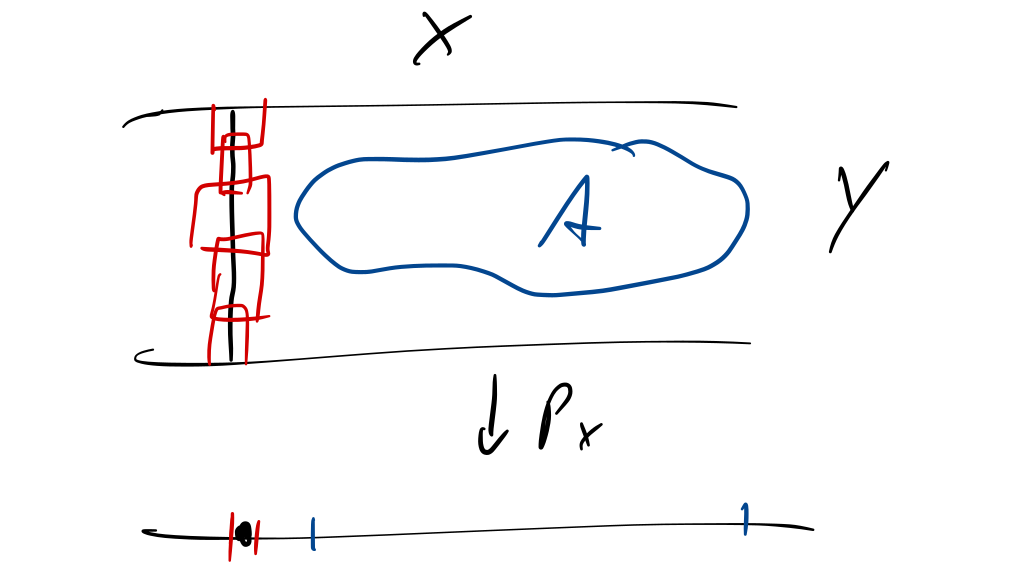
\includegraphics[scale=0.25]{figures/handdrawn/sketch-proof-thm-7.3.png}
        \caption{Beweisskizze zu \autoref{thm:projektion-auf-x-ist-abgeschlossen-wenn-y-kompakt}}
    \end{figure}
\end{proof}
\begin{lemma}[Subbasis der Produkttopologie]\label{lm:subbasis-der-produkttopologie}
    Seien $X,Y$ topologische Räume. Die Menge
     \[
    \mathcal{S} = \left \{U\times Y, X\times V \mid  U\subset X \text{ offen}, V\subset Y \text{ offen}\right\} 
    .\] 
    ist eine Subbasis der Produkttopologie.
\end{lemma}
\begin{proof}
    Sei $W\subset X\times Y$ offen. Dann gibt es nach der Definition der Produkttopologie $U_i\subset X, V_i\subset Y$ offen mit
    \[
        W = \bigcup_{i \in  I} (U_i \times V_i)
    .\] 
    Also ist bereits
    \[
        W = \bigcup_{i \in  I} ((U_i\times Y) \cap (X\times V_i))
    .\] 
    eine Vereinigung endlicher Schnitt von unseren Subbasiselementen. \\
    Umgekehrt ist klar, dass alle Elemente aus $\mathcal{S}$ auch offene Mengen in der Produkttopologie sind, da $\mathcal{S} \subset \mathcal{B}$.
\end{proof}
\begin{theorem}[Universelle Eigenschaft des Produkts]\label{thm:universelle-eigenschaft-endliches-produkt}
    Seien $A,X_1,X_2$ topologische Räume sowie $f_i: A \to  X_i$. Dann ist die Abbildung
        \begin{equation*}
            (f_1\times f_2) =: f \left| \begin{array}{c c l} 
        A & \longrightarrow & X_1\times X_2 \\
        a & \longmapsto &  (f_1(a),f_2(a))
        \end{array} \right.
    \end{equation*}
    stetig genau dann, wenn $f_1,f_2$ stetig sind. 
    \[
    \begin{tikzcd}
        & & X_1 \\
        A \ar[dashed]{r}{f} \ar[bend left = 30]{rru}{f_1} \ar[swap, bend right = 30]{rrd}{f_2} & X_1\times X_2 \ar{ur}{p_1} \ar{dr}{p_2} \\
                                                                              & & X_2
    \end{tikzcd}
\]
\end{theorem}
\begin{proof}
    Es ist $f_i = p_i \circ  f$. Ist $f$ stetig, so ist  $f_i$ stetig als Verknüpfung stetiger Funktionen. \\
    Angenommen, es sind $f_1,f_2$ stetig. Wir müssen zeigen, dass für alle $U_1\times U_2\subset X_1\times X_2$ mit $U_i\subset X_i$ offen auch $f^{-1}(U_1\times U_2)$ offen ist. Hierzu stellen wir aber fest, dass
    \[
        f^{-1}(U_1\times U_2) = f_1^{-1}(U_1) \cap  f_2^{-1}(U_2)
    .\] 
    offen ist.
\end{proof}
\begin{example}
    \begin{enumerate}[a)]
        \item Wir behaupten, dass
            \[
                \R^{n+1} \setminus \left \{0\right\} \cong S^n \times (0,\infty) \cong S^n \times \R
            .\] 
            ist. Betrachte hierzu
                \begin{equation*}
                \varphi : \left| \begin{array}{c c l} 
                    \R^{n+1}\setminus \left \{0\right\}  & \longrightarrow & S^n\times (0,\infty) \\
                    x & \longmapsto &  \left( \frac{x}{\lVert x \rVert _2}, \lVert x \rVert _2 \right) 
                \end{array} \right.
            \end{equation*}
            Wir sehen nun mit der universellen Eigenschaft sofort, dass es sich um eine stetige Abbildung handelt. Zudem haben wir die Umkehrfunktion
                \begin{equation*}
                \begin{array}{c c l} 
                    S^n \times (0,\infty) & \longrightarrow & \R^{n+1}\setminus \left \{0\right\}  \\
                    (y,t) & \longmapsto &  t\cdot y
                \end{array}
            \end{equation*}
            Wir müssen noch prüfen, dass diese stetig ist (Übung), dann haben wir einen Homöomorphismus.
        \item $S^1\times S^1$ ist ein Torus. Betrachte hierzu
               \begin{equation*}
               \varphi : \left| \begin{array}{c c l} 
                   [0,1]^2 & \longrightarrow & S^1 \times S^1 \\
                   (s,t) & \longmapsto &  (e^{2\pi is}, e^{2\pi it})
               \end{array} \right.
           \end{equation*}
           $\varphi $ ist stetig und erfüllt $\varphi (s,0) = \varphi (s,1)$ sowie $\varphi (0,t) = \varphi (1,t)$. Also faktorisiert $\varphi $ wie gewünscht als
           \begin{tikzcd}
               \left[0,1\right]^2 \ar{r}{\varphi } \ar{d} & S^1 \times S^1  \\
               \left[0,1\right]^2 / \sim \ar[swap]{ur}{\varphi '}
           \end{tikzcd}
           wobei $\sim $ die Relation ist, die wir für die Konstruktion des Torus verwendet hatten. $\varphi '$ ist stetig und surjektiv nach der Universellen Eigenschaft, und wir sehen leicht, dass $\varphi '$ injektiv ist. Also ist $\varphi '$ stetig und bijektiv. Nun ist aber $[0,1]^2$ kompakt und $S^1 \times S^1$ Hausdorff (z.B. als metrisierbare Teilmenge von $\R^2 \times \R^2$), und somit ist $\varphi '$ ein Homöomorphismus nach \autoref{cor:stetige-bijektion-von-kompaktem-raum-in-hausdorff-raum-ist-homöomorphismus}

           \begin{minipage}{\textwidth}
               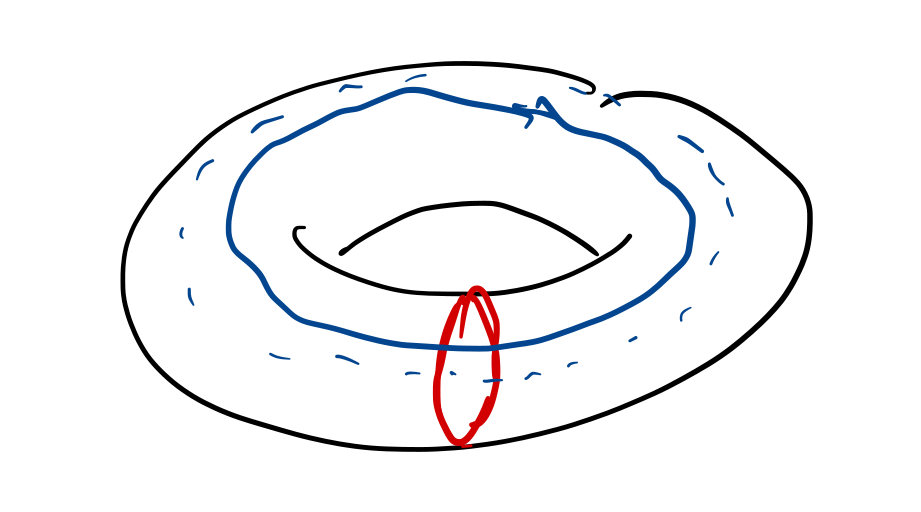
\includegraphics[scale=0.25]{figures/handdrawn/sketch-torus-als-produkt-von-s1-und-s1.png}
               \captionof{figure}{Die Einbettung von $T\cong S^1 \times  S^1$}
           \end{minipage}
    \end{enumerate}
\end{example}
\begin{corollary}[Komponente eines Produkts]\label{cor:topologischer-raum-ist-natürlich-in-seinem-produkt-enthalten}
    Seien $X,Y$ topologische Räume sowie  $y\in Y$. Dann ist $X\cong X\times \left \{y\right\} \subset X\times Y$ mittels $x \mapsto (x,y)$.
\end{corollary}

\begin{proof}
    Nenne diese Abbildung $f$, also
        \begin{equation*}
        f: \left| \begin{array}{c c l} 
        X & \longrightarrow & X\times Y \\
        x & \longmapsto &  (x,y)
        \end{array} \right.
    \end{equation*}
$f$ ist stetig, da sowohl  $\id_X$ als auch
    \begin{equation*}
    c_Y: \left| \begin{array}{c c l} 
    X & \longrightarrow & Y \\
    x & \longmapsto &  y
    \end{array} \right.
\end{equation*}
stetig sind (mit universeller Eigenschaft). $f$ faktorisiert nun über  $X\times \left \{y\right\} \subset X\times Y$ und $f: X \to  X\times \left \{y\right\} $ ist offensichtlich bijektiv. Wir müssen also noch zeigen, dass $f$offen ist. \\
Sei  $U\subset X$ offen, dann ist $U\times Y \subset X\times Y$ offen. Es ist zudem
\[
    f(U) = U\times \left \{y\right\}  = U\times Y \cap  X \times \left \{y\right\}  \subset X\times \left \{y\right\} 
.\] 
in $X\times \left \{y\right\} $ offen.
\end{proof}
\begin{theorem}[Produkteigenschaften]\label{thm:produkte-erhalten-hausdorff-und-kompaktheit}
    Seien $X,Y$ topologische Räume.
\begin{enumerate}[1)]
        \item Sind $X$ und  $Y$ Hausdorffsch, so auch  $X\times Y$
        \item Sind $X$ und $Y$ kompakt, so auch  $X\times Y$.
    \end{enumerate}
\end{theorem}
\begin{proof}
    \begin{enumerate}[1)]
        \item Seien $(x,y) \neq  (x',y' \in X\times Y$. Dann ist $x\neq x'$ oder $y\neq y'$. OBdA sei $x\neq x'$. Dann existieren $U,U'\subset X$ offen mit $x\in U, x'\in U'$ und $U\cap U' = \emptyset$, weil $X$ Hausdorffsch. Dann sind
            \[
                (x,y)           \in  U\times Y \qquad (x',y') \in U' \times Y
            .\] 
    jeweils offen, und ihr Schnitt ist
    \[
        (        U\times Y) \times (U'\times Y) = (U\cap U') \times Y = \emptyset
    .\] 
    Also ist $X\times Y$ Hausdorffsch.
\item Wir wollen den \nameref{thm:alexander} (\ref{thm:alexander}) verwenden. Sei $\mathcal{U}$ eine offene Überdeckung von  $X\times Y$ mit Elementen der Form $U\times Y$ oder $X\times V$. Sei
    \[
    W = \bigcup_{U\times Y \in \mathcal{U}} U \subset X \qquad W' = \bigcup_{X\times V \in \mathcal{U}} V \subset Y  
    .\] 
    Ist $W = X$, so existiert eine endliche Teilüberdeckung von  $\left \{U \mid  U\times Y \in \mathcal{U}\right\} $ durch $U_1,\ldots,U_n$. Dann ist bereits
    \[
    \left \{U_i \times Y \mid  i=1,\ldots,n\right\} 
    .\] 
    eine endliche Teilüberdeckung von $X\times Y$. Für $W' = Y$ verfahren wir genauso. Ist  $W \neq  X$ und $W'\neq Y$, so existiert $x\in X \setminus W, y\in Y \setminus W'$. Dann ist $(x,y)$ aber nicht von  $\mathcal{U}$ überdeckt, weil er von keinem $U\times Y$ und von keinem $X\times V$ überdeckt wird, \contra. \\
    Also finden wir in beiden Fällen eine endliche Teilüberdeckung.
    \end{enumerate}
\end{proof}
\begin{remark}
    Der Beweis geht auch ohne den \nameref{thm:alexander}. Viel leichter: Es genügt, offene Überdeckungen bezüglich einer Basis zu betrachten (Spezialfall von Alexander, leicht zu zeigen), dann verfahren wir wie folgt: \\
    Sei $\mathcal{U}$ eine Überdeckung von $X\times Y$ mit Elementen aus $\mathcal{B}$. Dann gibt es eine endliche Teilüebredckung von $X\times \left \{y\right\} $. Sei diese $\left \{U_i^y \times V_i^y\right\} i=1^{n_y}$. Setze
    \[
        V_y := \bigcap_{i=1} ^{n_Y} V_i^{y}
    .\] 
    Dann ist dies eine Überdeckung von $X\times V_y$. Die $V_y$ bilden nun eine offene Überdeckung von  $Y$, also finden wir wieder eine endliche Teilüberdeckung durch  $V_{y_1}, \ldots, V_{y_n}$. Da wir aber die $X\times V_{y_i}$ jeweils endlich überdeckt haben, können wir nun auch $X\times Y$ endlich überdecken.

    \begin{minipage}{\textwidth}
        \centering
        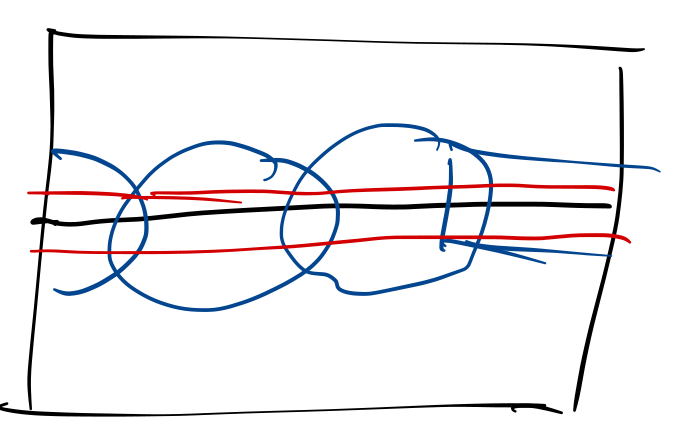
\includegraphics[scale=0.25]{figures/handdrawn/beweis-tychonoff-ohne-satz-von-alexander}
        \captionof{figure}{Skizze für den alternativen Beweis von \autoref{thm:tychonoff} für endlich viele Räume.}
    \end{minipage}
\end{remark}
\begin{ddefinition}[Produkt endlich vieler Mengen]\label{def:produkt-endlich-vieler-mengen}
Seien $X_1,\ldots,X_n$ topologische Räume. Dann definieren wir ihr Produkt rekursiv durch
\[
    X_1\times \ldots\times X_n := (X_1\times \ldots\times X_{n-1})\times X_n
.\] 
\end{ddefinition}

\begin{lemma}[Basis des Produktes]\label{lm:basis-des-produktes-zweier-räume}
    Seien $X,Y$ topologische Räume mit Basen  $\mathcal{B}_X, \mathcal{B}_Y$. Dann ist
    \[
    \mathcal{B}_{X\times Y} := \left \{U\times V \mid  U\in \mathcal{B}_X, V\in \mathcal{B}_Y\right\} 
    .\] 
    eine Basis der Topologie auf $X\times Y$.
\end{lemma}
\begin{corollary*}[Basis endlicher Produkte]\label{cor:basis-endlicher-produkte}
    Die Mengen $U_1\times U_2\times \ldots.\times U_n$ mit $U_i\subset X_i$ offen sind eine Basis der Topologie auf $X_1\times \ldots\times X_n$. \\
    Insbesondere ist die Topologie unabhängig von der Klammerung.
\end{corollary*}
\begin{proof}
    Setze $\mathcal{B}_{X_i} = \mathcal{O}_{X_i}$.
\end{proof}
\begin{proof}[Beweis von \autoref{lm:basis-des-produktes-zweier-räume}]
    Seien $W\in X, W'\subset Y$ offen. Dann existieren $U_i \in \mathcal{B}_X$ sowie $V_j \in \mathcal{B}_Y$ mit
    \[
    W = \bigcup_{i \in  I} U_i \qquad W' = \bigcup_{j\in J} V_j 
    .\] 
    Dann ist bereits:
    \[
    W \times W' = \bigcup_{\substack{i\in I \\j\in J} } U_i \times V_j
    .\] 
    Ist nun $A\subset X\times Y$ beliebig offen, so gilt
    \[
    A = \bigcup W_i \times W_i' = \bigcup  \bigcup_{\substack{i\in I\\j\in J}  } U_i \times V_j
    .\] 
    Umgekehrt ist klar, dass die $U_i\times V_j$ offen in der Produkttopologie sind.
\end{proof}
\begin{remark*}
    Im Beweis wurden - der Einfachheit halber - manche Indexmengen weggelassen. Es ist aber leicht einzusehen, dass es sich hierbei nur um ein formales Detail handelt.
\end{remark*}

\begin{remark*}
    Eigentlich haben wir \csname ifmkessler@fancythm@lecturenumbers\endcsname im Beweis des Korollars \else im Beweis von \autoref{cor:basis-endlicher-produkte} \fi die Aussage von \autoref{lm:basis-des-produktes-zweier-räume} für beliebig viele Räumen (endlich viele) benutzt. Man verallgemeinert das Lemma jedoch induktiv leicht auf endlich viele Räume:

\end{remark*}
\begin{proof*}[Beweis von \autoref{lm:basis-des-produktes-zweier-räume}]
    Den Fall $n=2$ verwenden wir als Induktionsanfang, er wurde bereits gezeigt. Seien nun $X_1,\ldots,X_n$ mit Basen $\mathcal{B}_i$ gegeben, dann wissen wir per Induktionsannahme bereits, dass 
    \[
    \mathcal{B}_{X_1\times \ldots\times X_{n-1}} := \left \{U_1\times \ldots\times U_{n-1}\mid U_i \in \mathcal{B}_i\right\} 
    .\] 
    eine Basis von $X_1\times \ldots\times X_{n-1}$ ist. Zudem ist $\mathcal{B}_n$ eine Basis von $X_n$ und somit ist
\[
    \begin{split}
        \mathcal{B}_{(X_1\times \ldots\times X_{n-1})\times X_n}:&= \left \{(U_1\times \ldots U_{n-1})\times U_n \mid  U_i \in \mathcal{B}_i\right\} \\
                                                                 &=\left \{U_1\times \ldots\times U_n \mid  U_i \in \mathcal{B}_i\right\} \\
                                                                 &=: \mathcal{B}_{X_1\times \ldots\times X_n}
    \end{split}
\]
eine Basis von $(X_1\times \ldots X_{n-1})\times X_n = X_1\times \ldots\times X_n$ und der Induktionsschritt ist erbracht.
\end{proof*}

\begin{theorem}[Diagonaleigenschaft]\label{thm:raum-ist-hausdorff-gdw-diagonale-abgeschlossen}
    Sei $X$ ein topologischer Raum. Dann ist  $X$ Hausdorffsch, genau dann, wenn
     \[
         \Delta_X := \left \{(x,x) \mid  x\in X\right\}  \subset X\times X
    .\] 
    abgeschlossen ist.
\end{theorem}
\begin{notation*}
    Wir nennen $\Delta_X\subset X^2$  die \vocab{Diagonale von $X$}.
\end{notation*}
\begin{proof}
'$\implies$' Nimm an, dass $X$ Hausdroffsch ist und sei  $(x,y) \in X \times X \setminus \Delta_X$, d.h. $x\neq y$. Dann existieren $x\in U_x,y\in U_y$ offen (in $X$), sodass  $U_x \cap  U_y = \emptyset$. Also ist
    \[
        (x,y)\in     U_x\times U_y \subset X\times X \setminus \Delta_X
    .\] 
    , denn wenn $(a,b) \in U_x \times U_y$, dann ist $a\neq b$. Also ist  $X\times X \setminus \Delta_X$ offen nach Definition. \\
    '$\impliedby$'    Nimm nun an, dass die Diagonale abgeschlosen ist. Seien $x,y\in X$ mit $x\neq y$ beliebig. Dann ist
    \[
        (x,y) \in X\times X \setminus \Delta_X = \bigcup_{i\in I} U_i \times V_i 
    .\] 
    Also ist $(x,y) \in U\times V \subset X\times X\setminus \Delta_X$ für eine Wahl von $U,V$. Dann ist aber  $x\in U, y\in V$ sowie $U\cap V = \emptyset$, denn wenn $a\in U\times V$, so $(a,a) \in U\times V \cap  \Delta_X = \emptyset$, \contra.
\end{proof}
\begin{definition}[Produkte beliebiger Mengen]\label{def:produkt-beliebiger-mengen}
    Sei $\left \{X_i\right\} _{i \in I}$ eine Familie topologischer Räume. Die Produkttopologie auf
    \[
        \prod_{i\in I} X_i := \left \{(x_i)_{i\in I} \mid  x_i \in X_i\right\} 
    .\] 
    ist die Topologie erzeugt von der Subbasis
    \[
    \mathcal{S}  := \left \{U_j \times  \prod_{i\neq j} X_i \mid  j\in I, U_j \subset X_j \text{ offen}\right\} 
    .\] 
\end{definition}
\begin{remark}
    \begin{itemize}
        \item 
    $\mathcal{S}$ ist wirklich nur eine Subbasis. Eine Basis ist gegeben durch
    \[
        \mathcal{B} := \left \{\prod_{j\in J} U_j \times \prod_{i\in I \setminus J} X_i \mid  J\subset I \text{ endlich}, U_j \subset X_j \text{ offen}\right\} 
    .\] 
    d.h. wir dürfen bei endlich vielen Faktoren eine endliche Teilmenge wählen, und wählen in den restlichen Faktoren den ganzen Raum
\item Ist $I$ endlich, so stimmt dies mit der vorherigen Definiton überein, weil wir für die Basis jeweils  $J = I$ wählen können.
\item \Warning Ist  $I$ unendlich, so ist im Allgemeinen
     \[
    \prod_{i\in I} U_i
    .\] 
    mit $U_i \subset X_i$ offen \underline{nicht} offen. 
    \end{itemize}
\end{remark}
\begin{remark*}[Mengentheorie-Spam]
    \begin{itemize}
        \item Wir benötigen das Auswahlaxiom, um einzusehen, dass obiges Produkt überhaupt nichtleer ist, sofern keiner der Faktoren leer ist. Formal ist das Produkt der $X_i$ nämlich definiert als
     \[
         \prod_{i\in I} X_i := \left \{f: I \to  \bigcup_{i\in I} X_i \mid \forall i\colon f(i) \in X_i \right\} 
    .\] 
    und das Auswahlaxiom besagt genau, dass es für jede solche Familie nichtleerere Mengene (mindestens) eine solche Funktion gibt (es ist also äquivalent dazu, dass die Produkte nichtleer sind).
\item Im Gegensatz zu dem, was in der Vorlesung genannt wurde, ist es kein Problem, wenn $I = \emptyset$, also die Familie leer ist. Dann ist nämlich
    \[
        \prod_{i\in I} X_i = \left \{f: \emptyset \to \emptyset \mid  \forall i\colon f(i)\in \emptyset\right\} = \left \{\emptyset\right\}  
    .\] 
    \underline{nicht} leer. (Hierzu sollte man sich klarmachen, dass eine Funktion  $f:A\to B$ eine Teilmenge von $A\times B$ war, sodass $\forall a\in A \;\exists !b \in B\colon (a,b) \in f$, und somit suchen wir eine Teilmenge $f\subset \emptyset\times \emptyset = \emptyset$). \\
    Auch die Topologie ist in diesem Fall wohldefiniert, weil die Subbasis wieder die leere Menge ist (nämlich eine Teilmenge von $\prod X_i = \left \{\emptyset\right\} $, und zwar $\left \{\emptyset\right\} $ selbst), und diese ist auch eine vollständige Topologie, weil unser topologischer Raum nur einen Punkt enthält (nämlich $\emptyset$). Wir erhalten also den einpunktigen topologischen Raum.
    \end{itemize}
\end{remark*}

